\documentclass[12pt,a4paper,oneside]{article}
\usepackage{amsmath,amsfonts,amssymb,amsthm}
\usepackage{cite}
\usepackage{algorithmic}
\usepackage{graphicx}


\usepackage{subfigure}
\bibliographystyle{plain}
\renewcommand{\algorithmicrequire}{\textbf{Input:}}
\renewcommand{\algorithmicforall}{\textbf{for each}}

\title{Path-set -- A Newer Platform for Genome Assembly With Mate-Pairs}
%%-- \usepackage[14pt]{extsizes}

\def\eps{\varepsilon}

\begin{document}

\maketitle

\begin{abstract}


One of the key advances that has led to a significant improvement 
in contig lengths has been mate pairs, which facilitate the assembly of repeating regions. 
In most current assemblers, mate-pair information has been used 
in  various post-processing steps to untangle the assembly graph or to link contigs
into scaffolds. These methods, although having different names, share the same
underlying mechanism with the mate-pair transformation procedure~\cite{Pevzner01b}:  finding a unique path between mate-pairs in the assembly graph and transforming 
mate-pairs into single long reads by filling the gaps between them. 
When multiple paths matching the insert size's range  exist between the left and right reads of a mate-pair,
 the traditional mate-pair transformation procedure fails and therefore the resulting assembly deteriorates as 
the variation of the insert size is high. 
Recently,~\cite{Medvedev11, Donmez11, Chikhi11} proposed similar platforms for genome assembly that incorporate 
the paired information in the graph structure rather than using it in the post-processing heuristics. However,
these methods face difficulties when the variation of the insert sizes is high. 
To facilitate this problem, instead of using mate-pairs reads directly, we transform them into 
edge-pairs and further, combine the ideas of mate-pair transformation, paired de Bruijn graph and 
de Bruijn graph structure to create the so-called Path-set graph platform for genome assembly.

\end{abstract}
\section{Introduction}



The current generation sequencing platforms such as ABI Solid, Illumina, 454 Life Science,
with short reads and high throughput allow genomes to be sequenced more quickly with lower cost and
has enabled new experimental opportunities to a variety of biological applications, including DNA methylation study, cancer research,
 ChIP-seq and whole transcriptome sequencing. However, as the sequencing technologies improves, 
the available sequenced data does not make the assembly task easier, if not harder. In fact, current genome 
assemblers face the challenge of assembling from reads of much shorter length (hundreds of 
nucleotides) comparing to longer reads in the previous Sanger sequencing platform
(thousands of nucleotides). In repeat-rich genomes, when the length of the repeat
is longer than twice the read length, correctly matching up its upstream and downstream regions is difficult.
Fortunately, all current sequencing platforms have been able to produce mate-pairs --
pairs of short reads between which the genomic distance (called the insert size) is approximately
known. Because insert sizes could be much longer than the read length, mate
pairs were able to span long repeats and could potentially match up the regions
surrounding a repeat. 


Mate-pair information has played an important role in 
most genomes projects and many current assemblers have  modules to incorporate mate-pair
information to improve the contigs length in a post-processing steps (mate-pair transformation 
in EULERSR~\cite{Chaisson08}, Breadcrumb in Velvet~\cite{Zerbino08}, Allpaths in ALLPATHS\cite{Butler08}, etc.). Albeit having 
different names, most of these modules rely on the same basic observation: If there is a unique
path in the assembly graph that connects the left and right reads of the mate-pair, the gap in the 
mate-pair can be filled in with the nucleotide sequence representing the found path. 
When multiple paths are found between the mate-pairs, it remains ambiguous which path 
should be used to filled in the gap. When the variation of insert size increases, 
the number of paths that match the possible values of the insert size will increase and
therefore, the mate-pair transformation efficiency (percentage of unique paths) decreases. Unfortunately,
current technologies have the variation in reads about 5\% of the insert size. 
Could the distance between reads be estimated exactly, the mate-pair transformation efficiency would 
increase and therefore improved the assembly. In the case when all the mate-pair transformations 
were successful, it would clearly create an upper bound for any repeat resolving methods using mate-pair. 



Only recently, \cite{Medvedev11} introduced the paired de Bruijn graph platform that 
incorporates mate-pair information in the graph structure rather than use 
them for the mate-pair transformation in the post-processing steps. \cite{Donmez11,Chikhi11} also
independently developed similar platforms for using mate-pairs. 
Unfortunately, the performance of these platforms deteriorates as
the variation of the insert size increases and undoubtedly, plays as a major obstacle for 
most current assembly methods using mate-pairs. 




The main contributions of this paper are as follow. In the method section, we  address
the variation of the insert size problem by transforming mate-pairs to edge-pairs (pair
of edges in the condensed de Bruijn graph). Using a collection of edge-pairs, we further combine the ideas of 
mate-pair transformation and paired de Bruijn graph to a single platform for genome assembly.
Namely, we present a basic data structure called path-set, which is a set of possible paths between edge-pairs,
and path-set graph to further extend path-sets into contigs. In the result section, we compare the 
performance of the path-set graph platform to most of the widely used assemblers on multiple E.Coli datasets.




\section{Methods}
\subsection{Basic Notations}
%define kmer, de bruijn graph, condensed de bruijn graph and mapping of a k-mer to the condensed
%de bruijn graph



Define a $k$-mer as a string of length  $k$. Given a $k$-mer $s=s_1\ldots s_k$, define 
$prefix(s) = s_1 \ldots s_{k-1}$  and $suffix(s) = s_2 \ldots s_k$. Given a set 
of $k$-mers $A$, the de  Bruijn graph $G$ is constructed with an edge $e=(u,v)$ for each $k$-mer
where $u$ and $v$ are the prefix and suffix of the $k$-mer respectively. The 
condensed de Bruijn graph $B$ is obtained by replacing every non-branching path in
$G$ by a single edge with length equal to the number of edges in the
corresponding path. Each edge in the condensed graph can be represented by an edge-list --- list of the normal de Bruijn graph edges. 
The length of a path in the condensed graph equals to sum of the length of all its edges. 



Each $k$-mer corresponds (maps) to an edge in the de Bruijn graph $G$ and therefore, uniquely identified by an 
edge and a position on that edge in the condensed graph $B$ (the position of the edge in the edge list). For example, Fig.~\ref{fig:edge1} is 
the condensed graph of the de Bruijn graph showed in Fig.~\ref{fig:nct}. 

A pair of $k$-mers $(a|b)$ is called a $(k,d)$-mer if they are at a distance $d$  in the original genome. We call $a$ and $b$: the left 
and the right $k$-mers of $(a|b)$ respectively.
Given parameters $d_0$ and $\Delta$, a $k$-pair $(a|b)$  is called a $(k,d_0,\Delta)$-mer of $S$ 
it is a  $(k,d)$-mer of $S$ where $d \in [d_0-\Delta, d_0+ \Delta]$. 
Given a set of $(k,d_0,\Delta)$-mers,  a pair of edges $(e_1,e_2)$ in the corresponding condensed de Bruijn graph  is called an edge-pair if 
there exists at least one $(k,d_0,\Delta)$-mers that its left and right $k$-mers map to position $p_1$, $p_2$ on $e_1$ and $e_2$ correspondingly. 



\begin{figure}
    \begin{center}
    \subfigure[De Bruijn Graph]{
    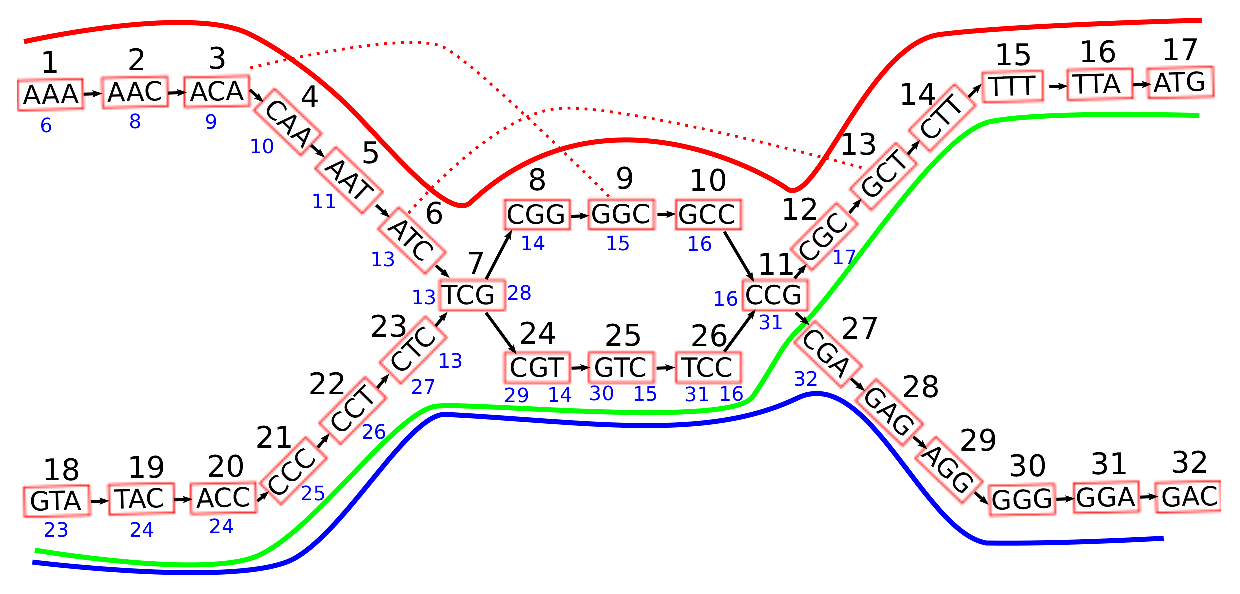
\includegraphics[scale =0.4] {fig/nct1.eps}
    \label{fig:nct}
    }
    \subfigure[Condensed de Bruijn Graph]{
    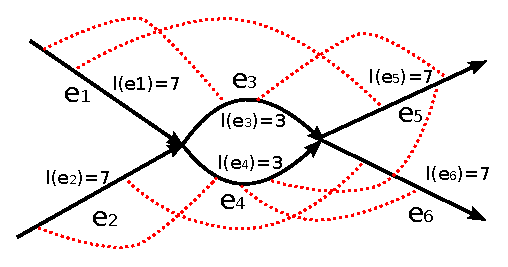
\includegraphics[scale =1] {fig/edge1.eps}
    \label{fig:edge1}
    }
    \caption{(a) De Bruijn graph and the corresponding mapping of mate-pairs. The number on top of each node is the node ID where the smaller number below each node 
shows the corresponding paired node. The bold red, blue and green sequences demonstrate how the genome traverses the graph.
(b) The condensed de Bruijn Graph --- non-branching paths of the graph in (a) correspond to condensed edges in this graph. The dotted red lines show
the edge-pairs information}
    \end{center}
\end{figure}



\subsection{From $(k,d, \Delta)$-mers to edge-pairs}

From the mate-pair reads where the mean insert size and its variation is known, we can generate a set of all $(k,d_0,\Delta)$-mers. This set can be easily transformed to 
a set of edge-pair using the above definition. Each edge-pair $(e_1,e_2)$ is represented as a triple $(e_1,e_2,\mathbf{h})$. In this triple, $\mathbf{h}$ is a 
histogram where $h(x)$ equals to the number of $(k,d_0,\Delta)$-mers that supports the \emph{genomic} distance $x$ between $e_1$ and $e_2$.
Namely, $h(x) = \Sigma I( d_0 +  p_{a_i} - p_{b_i} = x) $ where $p_{a_i}$, $p_{b_i}$ are
the positions that $a_i$ and $b_i$ map to $e_1$, $e_2$ respectively; $I$ is the indicator function; the summation is taken for all  $(k,d,\Delta)$-mers $(a_i|b_i)$ that 
 map  to  the edge-pair. Since the insert size follows a Gaussian-like distribution, with enough coverage the problem of estimating the distance less demanding  when 
the histogram contain a single distribution.. In this case
we can just use the peak of the distribution as the estimated distance. The complication raises when the histogram is a mixtures of  multiple distribution. In this case,
we choose a threshold and disregards the regions of the histogram where the values are below the threshold \footnote{An analytical formula for choosing the threshold 
would be beneficial}. The histogram results in one or more components, each component represents a tighter estimation of the distance between these edges. The original edge-pair
can be separated into multiple edge-pairs, each with a histogram supporting the distances for each component. Figure \ref{fig:distancehist}
shows an pair of edges $(e_1,e_2)$ that is traversed there times, each time passing $P_1$, $P_1$, and $P_3$. The first two of these repeats ($e_1 P_1 e_2$, $e_1 P_2 e_2$) have
similar length while  the last one ($e_1 P_3 e_2$) is well separated in length. Setting the threshold to 650 we can separate them into 2 components, one that has length 
varied from 130 to 147 and the other range from 156 to 165.  As a result, the original edge pair $(e_1, e_2,\mathbf{h})$ is transformed into two edge pairs: 
$(e_1,e_2,\mathbf{h_1})$ and $(e_1,e_2, \mathbf{h_2})$ where 
\[
h_1(x) = \left\{ 
\begin{array}{l l}
h(x) & \quad \text{if $x \in [130, 147]$}\\
0    & \quad \text{otherwise}\\
\end{array} \right.
\]
and 
\[
h_2(x) = \left\{ 
\begin{array}{l l}
h(x) & \quad \text{if $x \in [156, 165]$}\\
0    & \quad \text{otherwise}\\
\end{array} \right.
\]


While edge-pair is similar to mate-pair in that both of them  have a gap sequence between both ends, edge-pair possesses multiple advantages.
In edge-pair, the distance between both ends is better estimated and therefore more suitable for the previous methods for resolving repeats: mate-pair transformation~\cite{Pevzner01},
paired de Bruijn graph~\cite{Medvedev11}, paired graph~\cite{Donmez11}, etc. Moreover, since the edge-pairs set  is a compact representation of the original mate-pairs data, many 
redundant operations could be omitted directly, for instances, in mate-pair transformation, multiple function calls for mate-pairs that map the same pair of condensed edges can 
be replaced by a single mate-pair transformation on the corresponding edge-pair. 

Edge-pair data can be adapted into  most previous methods  that are susceptible to the variation of the insert size of mate-pairs. While the use of 
edge-pair in mate-pair transformation methods is straightforwards, the use of edge-pair in the paired de Bruijn graph requires some adjustments in 
the way the graph is constructed as the length of both ends of edge-pair are usually not equal. In the next section, rather than focusing 
on the use of edge-pairs and adapt it to each of the previous repeat resolving methods individually,  we combine  mate-pair 
transformation with an ad hoc version of paired de Bruijn graph on edge-pairs to build a more advanced platform: \emph{path-set} graph. 



\begin{figure}
    \begin{center}
    \subfigure[]{
    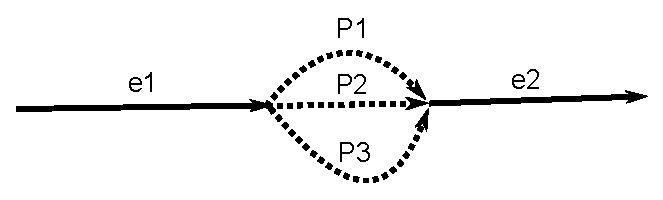
\includegraphics[scale =1] {fig/distancehist.eps}
    \label{fig:distancehist}
    }
    \subfigure[]{
    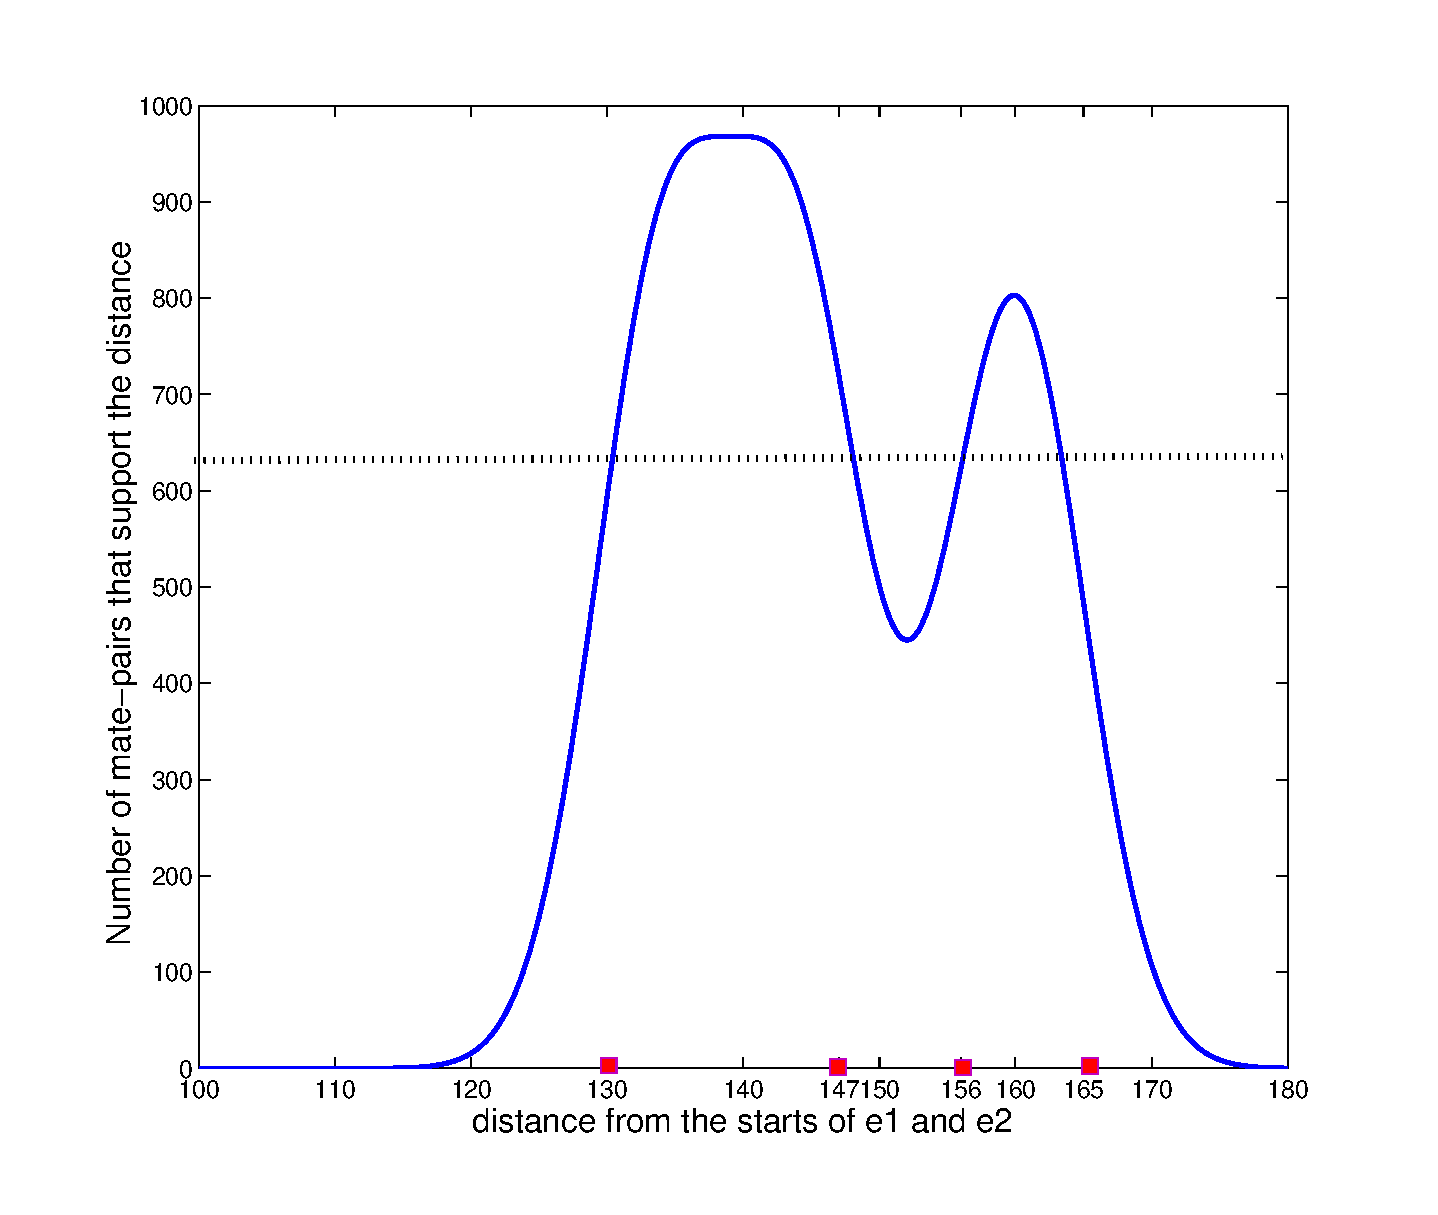
\includegraphics[scale =0.3] {fig/distancehistb.eps}
    \label{fig:distancehistb}
    }
    \caption{(a). The sequence traverses from $e_1$ to $e_2$ by 3 paths: $P_1$, $P_2$, and $P_3$. The length of $e_1$, $P_1$, $P_2$, and $P_3$ is 100, 34, 40 and 60 correspondingly. 
    (b) The histogram of mate-pairs that support 3 possible distances. Setting the threshold to 600, we obtained two separated components, one from 130 to 147 that supports 
    the traversal via paths $P_1$ and $P_2$ while the other component (from 156 to 165) that supports the traversal through path $P_3$.}
    \end{center}
\end{figure}


\subsection{Adapting edge-pairs to mate-pair transformation and paired de Bruijn graph --- Path-set and Path-set Graph}

\textbf{Path-set.}
Similar to the classic mate-pair transformation procedure, for each mate-edge $(e_1, e_2,\mathbf{h})$ we also look for paths between $e_1$
and $e_2$ that have length in the valid range of $\mathbf{h}$. Essentially, this amounted to transforming an edge-pair into long found path and
thus equivalent to having a much longer reads.  In different from the previous approach, where the procedure fails when there are multiple paths that match
the distance's range , we store all paths that correspond to possible traversals from edge $e_1$ to $e_2$ that match the distance constrain into a
structure called \emph{path-set} (a set of paths). For example, in Fig.~\ref{fig:edge1}, edge pair $(e_1, e_5)$ can be transformed to a path-set 
containing two paths $PS = \{e_1e_3e_5, e_1e_4e_5\}$


Path-sets have two important properties that make it useful: (a) path-sets are not intersected, (b) each path-set contains at least one 
path that is present in the genome. Theoretically, it may exist 
an exponential number of such paths in the graph and  an naive search for all paths between two nodes in the graph that
has a certain length is computationally expensive. In the appendix, we describe an algorithm with polynomial time and space for finding and
storing these paths. 


\textbf{Path-set Processing}.
Path-set plays the role as a single long read when it contains
a single element (path). When the path-set contains more than a single path, it remains ambiguous which path should be followed and this is a result of
the following reasons: (1) There are multiple repeats with similar length that shares both ends of the edge-pairs and vary in between, (2) There is only one 
valid connection between the two edges of the edge-pair but because of the intervention of other repeats, multiple paths 
that match the distance can be found. Were the read length that could span all the gap between the edge-pairs available, all path-set would 
simply be singletons and provides an upper bound for any repeats resolution approaches using only mate-pairs. Given a collection of path-sets obtained
from edge-pairs, we now use  the paired de Bruijn graph and the underlying de Bruijn graph structure to increase the number of path-set and
reduce the number of paths in each path-set while keeping the two basic properties of the path-sets.

\textbf{(a) Using the de Bruijn graph for path-set splitting}.
Initially, using the graph structure, we want to separate the path-sets into multiple non-disjoint path-sets while remaining their two basic 
properties. The goal is to distinguish repeats that share the both end edges but have variations in between. A path $P$ is called a mandatory
path if it  corresponds to a sequence that is present in the genomes. Intuitively, if all members of a path-set $PS$ are mandatory paths, we 
can split this path-set into multiple path-sets, each contains a single mandatory path. Even when we can not separate each path-sets into all
singletons, it is still helpful to divide them into multiple non-disjoin path-sets to reduce the ambiguity of traversal in each path-set.

A pair of edge $(e_i, e_j)$ is called a constraint of $e^*$ if $e^*$ lies between $e_i$ and $e_j$ for any 
covering tour of the graph, and $e^*$ is called a bridge\footnote{Note that this terminology is not related to the 
common meaning of \emph{bridge} in graph theory} of the constraint $(e_i, e_j)$.
In other words, all paths that can traverse $e^*, e_i, e_j$  have the following forms $e_i \ldots e^* \ldots e_j$ and we call them the constraint paths of edge $e^*$. 
Two bridge $e^*_1$   and $e^*_2$ (if exists) of the same constraint $(e_i, e_j)$ are called independent  if none of the constraint paths of $e^*_1$ 
contains $e^*_2$ and vise versa. For example, in Fig.~\ref{fig:bridge}, $(e_1,e_7)$ is a constraint of $e_2, e_3, e_5, e_6$; these four edges are called bridges. Among
them, $e_2$ and $e_3$, $e_5$ and $e_6$ are independent. 

If a path-set contains all paths that connects the start edges to the ends edges, we can find a maximum set of edges in these paths, such that they are pairwise independent and 
transform that path-set to multiple non-disjoint path-sets, each contains the constraint paths of an edge in the chosen set. 
\begin{figure}
    \begin{center}
    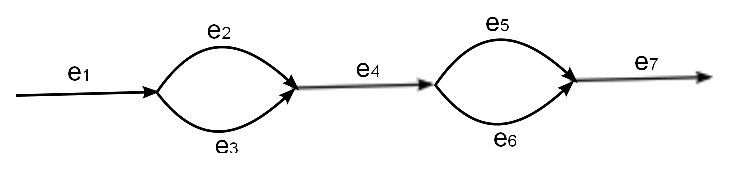
\includegraphics[scale =1] {fig/bridge.eps}
    \label{fig:bridge}
    \caption{ The path-set corresponding to the edge pair $(e_1, e_7)$ contains 4 paths $PS= \{e_1e_2e_4e_5e_7,e_1e_3e_4e_5e_7, e_1e_2e_4e_6e_7, e_1e_3e_4e_6e_7\}$. 
        --- all possible connection from edge $e_1$ to $e_7$. Edges $e_2$ and $e_3$ are independent bridges and therefore, $PS$ can be split into 2 path-sets: 
    $PS_1 =\{ e_1e_2e_4e_5e_7, e_1e_2e_4e_6e_7 \},  PS_2 =\{ e_1e_3e_4e_5e_7, e_1e_3e_4e_6e_7 \}$ }
    \end{center}
\end{figure}

\textbf{(b) Using edge-pairs to remove invalid paths in path-sets  --- An ad hoc Paired de Bruijn Graph Approach.}
Since not all paths in each path-set are required to appear in the genome, we  can remove the paths that are not supported by mate-pair information (edge-pairs). Edge $e_i$ is called 
extendible by $e_j$  if the following conditions hold: (1) if $e_j$ follows $e_i$ in the graph.
(2) There exist mate-pairs $(e_i, e^*_i, \mathbf{d_i})$\footnote{Note that after the mate-pair transformation procedure, the 
histogram in the edge-pair can be replaced by a set of possible distances ($\mathbf{d_i}$)}  and $(e_j, e^*_j,\mathbf{d_j})$ such that 
either $e^*_i = e^*_j$ and $d_i + l(e_i) = d_j$ 
or $e^*_j$ follows $e^*_i$ and $d_i + l(e_i) = d_j - l(e^*_j)$, where $d_i \in \mathbf{d_i}, d_j \in \mathbf{d_j}$. (3) There exist mate-pairs $(e^*_i, e_i, \mathbf{d_i})$
 and $(e^*_j, e_j,\mathbf{d_j})$ such that 
either $e^*_i = e^*_j$ and $d_i + l(e^*_i) = d_j$ 
or $e^*j$ follows $e^*_i$ and $d_i + l(e_i) = d_j - l(e^*_j)$, where $d_i \in \mathbf{d_i}, d_j \in \mathbf{d_j}$. A path $P= e_i e_{i+1} \ldots e_{i+t}$ is called a supported 
path if edge $e_{j}$  is extendible by $e_{j+1}, \forall j = 1..t-1$ and if the distance between any pair of edges $e_m$, $e_n$  in the path falls in 
the insert-size range, there exists an edge-pair of $(e_m,e_n)$ that supports the distance (in the path) from the starts $e_m$ to $e_n$.


\textbf{Path-set Graph}

Given a collection of path-sets generated from mate-pairs  where 
each path-set contains at least one path that is present in the genome and two different path-sets
do not have any path in common, the problem of assembling the genome from this collection is similar to 
the traditional genome assembly from single reads. Below, we define the path-set graph, namely the 
connection between path-sets to get longer contigs. 





Path $p_1$ is an absolute prefix of path $p_2$ if $p_2$ can be obtained from $p_1$ by
concatenating some non-zero-length path $p'$
to the end/start of $p_1$. A path $p'_2$ follows a path $p'_1$ if they have the following form:
$p'_1 = e_1e_2\ldots e_k$ and $p'_2= e_2\ldots e_k \ldots e_{k+t}$ where $t \geq 0$. 
A path-set $C_1$ is called an absolute prefix of path-set $C_2$ if each path of $C_1$ is an absolute 
prefix of at least one path in $C_2$. The path-set graph is constructed from the collection of path-sets as follows: (1) Remove all
the absolute prefix path-sets. (2) Represent each remaining path-set as a node and form an edge from node $C_i \rightarrow C_j$ if
there exists paths $p_i \in C_i$ and $p_j \in C_j$ such that $p_j$ follows $p_i$.




Fig.~\ref{fig:edge1} illustrates the construction of the path-set graph for a toy example. In this example, there are 8 path-sets. After removing 
all the prefixes path-sets, 6 path-sets remains. Among them, there are 3 path-sets that contains 2 paths, and 3 path-sets are singletons. 
After using mate-pair information to remove invalid paths, we obtains all 6 singletons path-sets. The graph is now simple with 3 non-branching paths corresponding to 
3 contigs. 




Note that the path-set graph shares similarities with both the de Bruijn graph and the overlap graph. 
It is similar to the de Bruijn graph that the edge $PS_i \rightarrow PS_j$ represents a $t-1$ overlapping edges 
where $t$ is the number of a path in $PS_i$. It is similar to the overlap graph that the genome corresponds to 
a covering walk that covers all nodes in the graph. With the input as a set of all mate-pair, the path-set 
graph platform can be summarized as follows:



\begin{algorithmic}[1]
\REQUIRE Set of mate-pairs
\STATE Construct the de Bruijn graph from reads
\STATE Construct the condensed de Bruijin graph
\STATE Transform mate-pair into a collection of edge-pairs with better estimated distance.
\STATE Transform each edge-pair to path-set
\STATE \textbf{Foreach} path-set
\STATE  \hspace*{0.5cm} Split the path-set  by using  the graph structure
\STATE \hspace*{0.5cm} Remove invalid paths by using mate-pairs
\STATE Construct path-set graph and output contigs as non-branching paths.
\end{algorithmic}

\section{Results}


\begin{figure}
    \begin{center}
    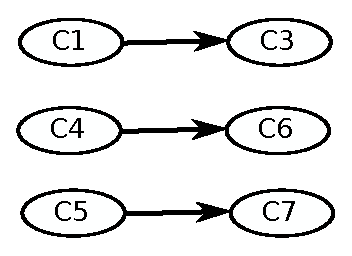
\includegraphics[scale =1] {fig/pathset7.eps}
    \label{fig:pathgraph1}
    \caption{The path-set graph constructed from the graph and mate-pair information in figure 1. Initially there are 8 path-sets: 
    $C_1= \{ e_1e_3e_5, e_1e_4e_5\}$,  $C_2= \{ e_1e_3\}$,$C_3= \{e_3e_5 \}$,$C_4= \{e_2e_3e_5,e_2e_4e_5 \}$,$C_5= \{e_2e_3e_6,e_2e_4e_6\}$,$C_6= \{e_4e_5 \}$,$C_7= \{e_4e_6 \}, C_8= \{e_2e_4 \}$.
Among them, $C_1, C_4$ and $C_5$ each contains two paths. Using the edge-pair information, we remove one invalid path in each of these path-sets. The path-set graph is then constructed
by firstly remove all prefixes path-sets ($C_2, C_8$). The path-set graph has 6 nodes and spell out 3 different contigs.  
}
    \end{center}
\end{figure}

% Similarly, the backward 
%path-set graph is constructed from $C$ as follows: (1) Remove all the absolute suffix path-sets. (2) Represent
%each remaining path-set as a node and form an edge from node $C_i \rightarrow C_j$ if there exists
%paths $p_i \in C_i$ and $p_j \in C_j$  in the following forms: $p_1 = e_{k} \ldots e_{k+1}\ldots e_{k+t}$ 
%and $p_2 = e_{k-t} e_{k} \ldots e_{k+1}\ldots e_{k+t}$ where
%$t \geq 0$.







\section{Discussion}

In this paper, we have presented the path-set graph --- a framework for assembling genomes using mate-pairs data. In stead of 
using mate-pair transformation on a set of mate-pair directly, which is computationally expensive and 
susceptible to failure when the insert size is high, we first transform them to edge-pairs. The distance between 
two edges in the edge-pairs can be estimated by using the distribution of all mate-pairs that maps to these condensed
edges. Furthermore, all mate-pair transformation operations for mate-pairs that correspond to the same 
edge-pair can be replaced by a single edge-pair transformation.
In different from the traditional mate-pair transformation approach, where a unique path between paired reads in the de Bruijn graph is required,
this new approach stores  all the paths in a structured called path-set, and latter using the paired information to remove invalid paths and utilizing 
the underlying graph structure to further distinguish the repeats in each path-set. We latter provide a way to construct the path-set graph to further 
extend path-set into contig. 

Multiple libraries with different insert size can also be utilized in the path-set graph approach. The paired information in different libraries can be used to 
remove invalid paths in each path-set. A further direction is to extend the path-set to a more stable platform that can work even in the case no path can be found 
between edge-pair --- which is caused by the gap in coverage in most current single cell dataset. 
 



\section{Appendix}










\bibliography{mybib}
\end{document}
